\section{Resultate}\label{resultate}
Es gibt x Lösungenansätze mit x varianten.  hier sind die Kompressionsraten der jeweils besten Varianten der Ansätze.\\
Bis auf den Lösungsansatz unter \ref{resultate:loesung0} Unterschiedliche Qualitätsstufen
\begin{table}
	\begin{tabular}{l|l}
		Ansätze & Kompressionsraten \\\hline
		Adaptives Subsampling & 11.6 \\
			
	\end{tabular}
	\caption{Tabelle der }
\end{table}

\subsection{Lösungsansatz: Adaptives Subsampling} \label{resultate:loesung0}
Im Ist-Zustand führt der JHelioviewer nach der Dekompression ein adaptives Subsampling durch. Dieser Lösungsansatz führt das adaptive Subsampling vor der Datenübertragung durch und Kodiert die Daten mit Rar anstatt mit Gzip. Eine genauere Beschreibung des Ansatzes ist im Abschnitt \ref{konzept:loesung0} zu finden.
\begin{figure}[!htbp]
	\center
	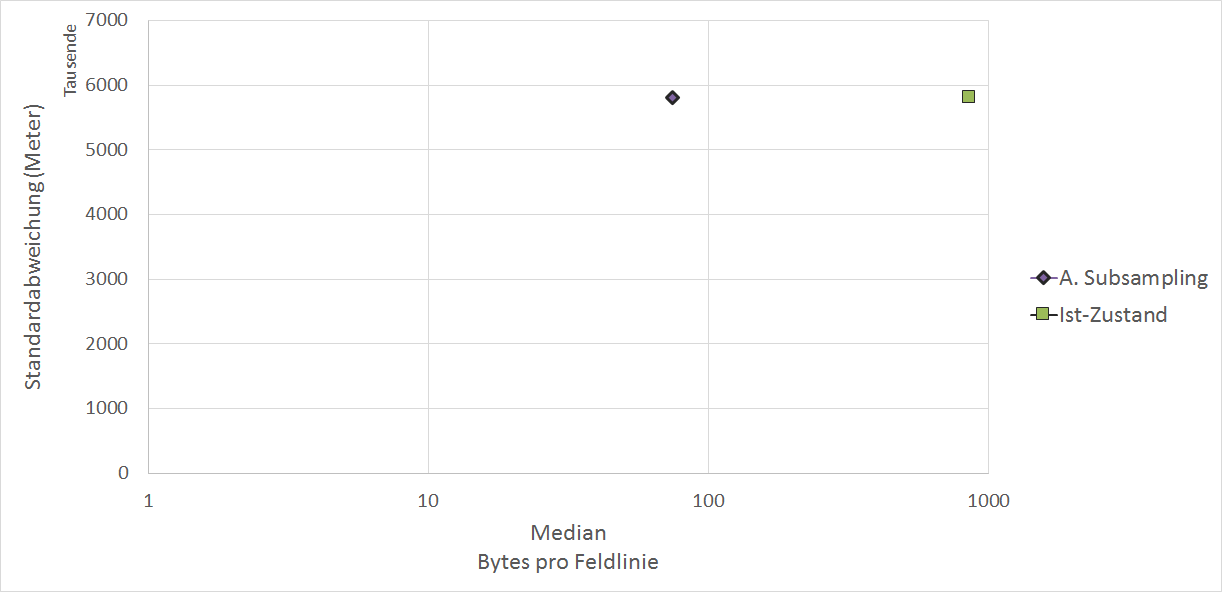
\includegraphics[width=0.8\textwidth,height=6cm,keepaspectratio]{./pictures/resultate/loesung0/loesung0_0.png}
	\caption{Vergleich des Lösungsansatzes: Adaptives Subsampling zur Ist-Kompression.}
	\label{resultate:loesung0:loesung0_0}
\end{figure}
%Grösse der DAtei
Wie im Diagramm \ref{resultate:loesung0:loesung0_0} erkennbar ist, braucht dieser Lösungsansatz deutlich weniger Speicher als die Ist-Kompression. Das Adaptive Subsampling reduziert deutlich die Anzahl Punkte, während die Rar eine bessere Kompression erbringt. Dieser Ansatz kann die Daten um Faktor $11.6$ besser komprimieren.\\
Die Komplexität dieses Ansatzes bleibt ist $O(n)$ ($n$ ist die Anzahl Punkte) und bleibt somit in der selben Komplexitätsklasse wie die Ist-Kompression. Dieser Lösungsansatz ist aber bei der Dekompression schneller, da $n$ etwa vier mal Kleiner ist. und ist som  Da bei der Dekompression $n$ etwa vier Mal weniger Punkte bearbeiten muss, ist die Dekompression sogar schneller als die Ist-Lösung.\\
\begin{figure}[!htbp]
	\center
	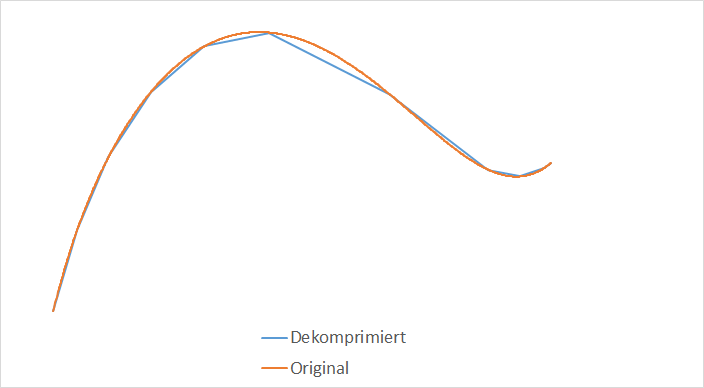
\includegraphics[width=0.8\textwidth,height=6cm,keepaspectratio]{./pictures/resultate/loesung0/loesung0_artefakte.png}
	\caption{Artefakte der Lösung 0}
	\label{resultate:loesung0:artefakte}
\end{figure}
Die Abbildung \ref{resultate:loesung0:artefakte} zeigt die Artefakte, die bei der Komprimierung der Lösung 0 entstehen. Es ist anzumerken, dass der Ist-Zustand die selben Artefakte aufweist.

\subsection{Lösungansatz: Diskrete Kosinus Transformation}
Lösungsvarianten
d
In den folgenden Abschnitten werden die Resultate verschiedener Varianten vorgestellt. Alle Varianten bestehen grob aus fünf Teilschritten: Einem Subsampling\footnote{siehe Abschnitt \ref{konzept:loesung1:subsampling}}, einer Folge von verschiedenen Transformationen, bei der eine die Diskrete Kosinus Transformation ist, Abspeicherung ins Fits Format\footnote{siehe Abschnitt \ref{konzept:loesung0:fits}} undeiner Quantisierung und einer Entropie Kodierung mit Rar\footnote{siehe Abschnitt \ref{konzept:loesung0:kodierung}}.\\
[\baselineskip]
In den Tests wurde eine lineare Quantisierung verwendet. Jeder DCT Koeffizient wird durch einen Faktor geteilt, der sich stetig ehöht. Zum Beispiel wird der erste Koeffizient durch zwei geteilt, der zweite durch Vier, der Dritte durch Sechse etc.  Die Kompressionsrate kann durch einen höheren oder tieferen Faktor gesteuert werden. Diese Quantifizierung ist nicht das Optimum. Eine bessere Quantifizierung wird für die beste Lösung ausgearbeitet.

\subsubsection{Variante: DCT}\label{resultate:dct}
Bild
verwendet als Transformation nur DCT. Eizige Veränderung, jeder Kanal wird mit 32 Bit Integer anstatt mit 16 Bit abgespeichert. DCT-Koeffizienten sind sonst zu gross.
\begin{figure}[!htbp]
	\center
	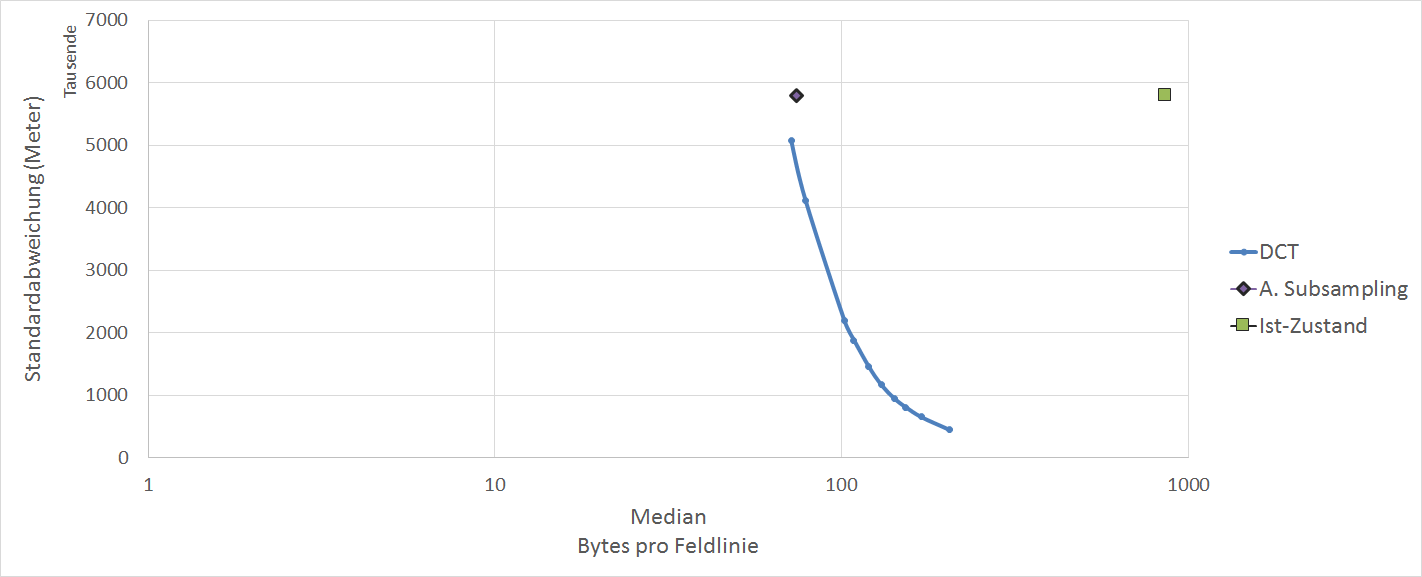
\includegraphics[width=0.8\textwidth,height=6cm,keepaspectratio]{./pictures/resultate/loesung1/loesung1-0/loesung1_0.png}
	\caption{Vergleich der DCT Kompression mit der Lösung0}
	\label{resultate:loesung1:dct:resultate}
\end{figure}
Die Abbildung \ref{resultate:loesung1:dct:resultate} zeigt den Vergleich der DCT Kompression mit der Lösung 0. Es ist deutlich zu erkennen, dass die Standardabweichung schnell steigt bei leicht sinkender Grösse. Der Maximale Fehler ist ist mehr als vier Mal grösser, als die der Lösungsvariante \ref{resultate:loesung0} steigt ebenfalls schnell und erreicht beim letzten Test eine höhe von $140'686'000$ Meter. Zum Vergleich: Der maximale Fehler der Lösung 0 ist mehr als vier Mal kleiner und liegt bei $30'014'000$ Meter.\\
\begin{figure}[!htbp]
	\center
	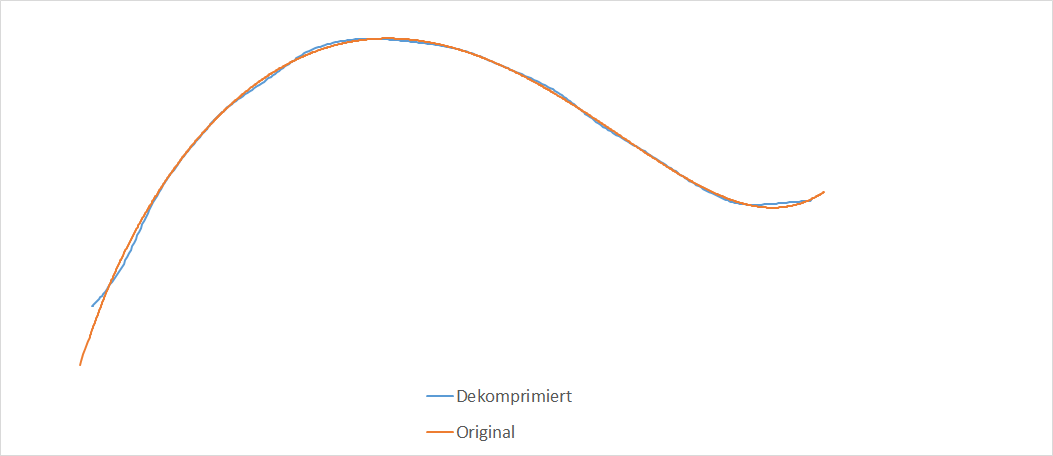
\includegraphics[width=0.8\textwidth,height=6cm,keepaspectratio]{./pictures/resultate/loesung1/loesung1-0/loesung1_0_artefakte.png}
	\caption{Artefakte der DCT Dekompression anhand Beispieldaten}
	\label{resultate:loesung1:dct:artefakte}
\end{figure}
Die Darstellung der Artefakte \ref{resultate:loesung1:dct:artefakte} zeigen das Problem: in den meisten Fällen kann die DCT die Feldlinie gut approximieren. Bei dieser Feldlinie wird der Anfang der Kurve nicht richtig dargestellt. Das ist ein typisches Problem der DCT. In diesem Fall wird für die Transformation angenommen, dass sich das Signal am Anfang und am Ende in umgekehrter Reihenfolge wiederholt \cite{wiki:dct}. Das führt am Anfang der Kurve zu einer grossen Spitze, welche sich nur durch sehr hochfrequente Schwingungen darstellen lässt.  Wenn diese Anteile durch die Quantisierung verschwinden, entstehen solche Artefatkte.\\
Eine Möglichkeit ist die Feldlinie um Punkte zu erweitern. Wenn die Feldlinie am Anfang und am Ende abflacht, sollte die resultierende Transformation weniger hochfrequente Schwingungen enthalten. Diese Variante wird im Abschnitt \ref{resultate:loesung1:dct:randbeh+byte} behandelt und führt zu einer deutlich besseren Approximation. Durch eine andere Darstellung der Daten kann das Problem ebenfalls gelöst werden. Diese Variante wird in den folgenden Abschnitten besprochen.

\subsubsection{Variante: Ableitung+DCT}\label{resultate:dct:ableitung_dct}
Bild
Bevor die Feldlinie Kosinus-Transformiert und Quantisiert wird, soll sie abgeleitet werden. Dämpfung der koeffizienten, die diskretisierten Koeffizienten sollten weniger speicherplatz verbrauchen. Mit der Ableitung soll das Randproblem dargestellt in \ref{resultate:loesung1:dct:artefakte} gelöst werden. Die Steigungen sind kleinere Zahlen, was an den Rändern keine grosse Spitze verursachen sollte. Der Nachteil ist, dass Ungenauigkeiten sich durch die Kurve durchziehen und summieren.\\
Damit die Ableitung umkehrbar ist, wird neu jeder Startpunkt der Feldlinie mit in die Fits Datei abgelegt. Die DCT-Koeffizienten werden mit 16 Bit Genauigkeit abgelegt.\\

\begin{figure}[!htbp]
	\center
	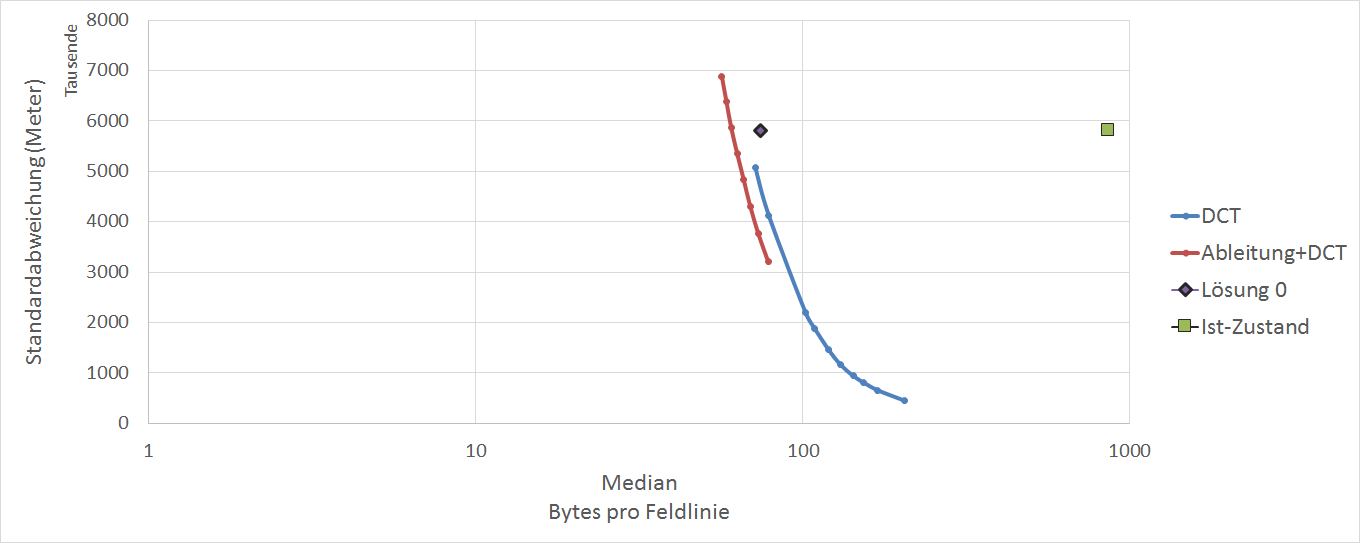
\includegraphics[width=0.8\textwidth,height=6cm,keepaspectratio]{./pictures/resultate/loesung1/loesung1-1/loesung1_1.png}
	\caption{Vergleich der DCT Kompression der Ableitung mit der DCT Kompression}
	\label{resultate:loesung1:dct:artefakte}
\end{figure}
Die abgeleiteten Feldlinien können sehr gut quantisiert werden. Im Vergleich zur Lösung 0 braucht diese Variante etwa $15$ Byte weniger um eine Feldlinie darzustellen. Durchschnittlich ist jetzt eine PFSS Simulation auf $72$ KiByte komprimiert. Die Ränder können dargestellt werden, eine Darstellung der Artefakte ist auf der Abbildung \ref{resultate:loesung1:dct:byte:artefakte} zu finden.\\
Die Feldlinien liegen meist auf einer Ebene im dreidimensionalen Raum. Wenn die X,Y und Z Kanäle Kosinus-Transformiert werden, ist die Information etwa gleichmässig auf den Kanälen verteilt. Eine Linie könnte sich durch weniger Kosinus-Funktionen approximieren lassen, wenn die Linie zuerst in ein lokales Koordinatensystem transformiert wird. Die Koordinatenachsen können für jede Linie so gelegt werden, dass der X und Y Kanal den grossteil der Informationen beinhalten. Es wird vermutet, dass für Approximation des X und Y Kanals mit etwa gleich viele Kosinus-Funktionen gebraucht werden, aber für den Z Kanal bedeutend weniger.

\subsubsection{Variante: Ableitung+PCA+DCT}
Bild
Die Principal Component Analysis (PCA)\cite{abdi2010principal} ist ein Verfahren aus der Statistik, welches Daten in ein neues koordinatensystem Transformiert. Dabei werden die Achsen so gelegt, dass die Daten entlang der ersten Achse die grösste Varianz aufweisen. Entlang der zweiten Achse, welche orthogonal zur ersten liegt, die zweithöchste Varianz etc. Wenn das Vefahren auf die Feldlinien angewandt wird, werden die Feldlinien in ein lokales System transformiert indem der Z-Kanal 0 ist, wenn die Feldlinie in einer Ebene liegt. Der Nachteil ist, dass für die Rücktransformation pro Feldlinie die Koordinatenachsen und die Koordinatenverschiebung abgespeichert werden.\\
Vor der DCT wird nun eine PCA durchgeführt. Die sechs Faktoren der neuen Koordinatenachsen werdenmit  16 Bit Genauigkeit in die Fits-Datei abgelegt und die drei Verschiebung-Faktoren mit 32 Bit.
\begin{figure}[!htbp]
	\center
	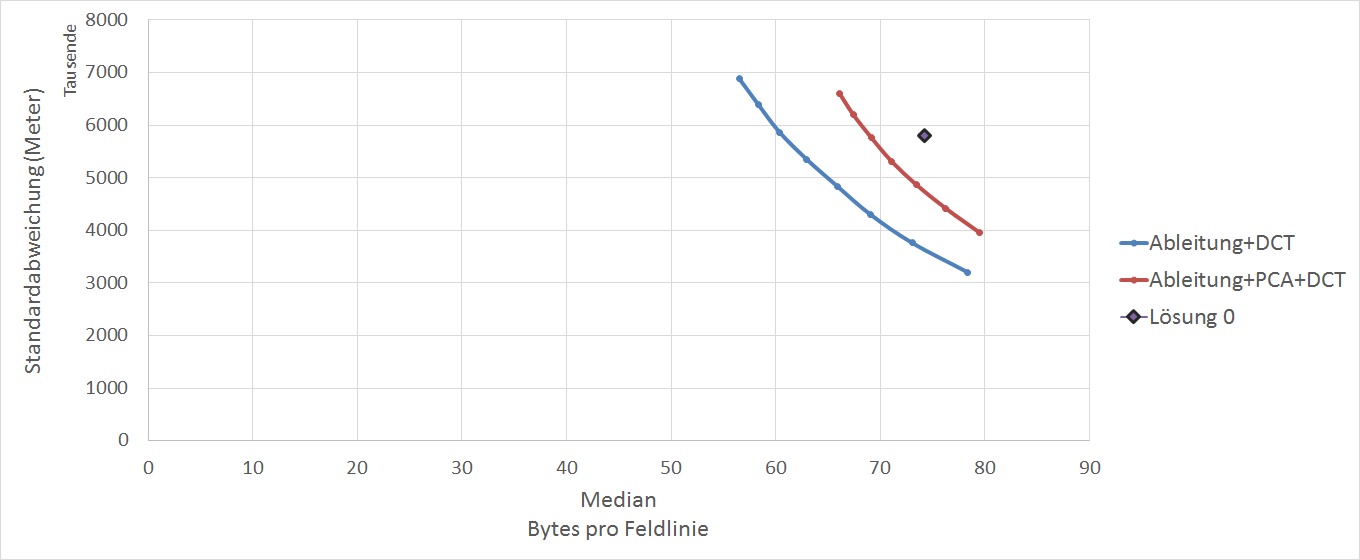
\includegraphics[width=0.8\textwidth,height=6cm,keepaspectratio]{./pictures/resultate/loesung1/loesung1-4/loesung1_4.png}
	\caption{Vergleich der PCA DCT Kompression der Ableitung mit der DCT Kompression der Ableitung}
	\label{resultate:loesung1:dct:pca}
\end{figure}
Der Vergleich \ref{resultate:loesung1:dct:pca} zeigt deutlich, dass sich der Mehraufwand nicht lohnt, obwohl die PCA vielversprechend scheint. Eine Feldlinie lässt sich mit 5 bis maximal 20 Kosinus-Funktionen pro Kanal approximieren. Durch die PCA-Transformation lässt sich das noch minim verkleinern, aber die zusätzlichen Informationen wie die Werte für neuen Koordinatenachsen und für die Verschiebung verbrauchen mehr speicher, als durch die Transformation gewonnen werden kann.\\
Die PCA-Variante könnte noch verkleinert werden. Die Verschiebung kann Quantisiert werden, oder man kann weniger Genauigkeit für die Koordinatenachsen verwenden. Die PCA-Variante ist aber nicht genauer wie die Ableitung+DCT Variante. Wie auch in \ref{resultate:loesung1:dct:pca} ersichtlich, ist die PCA-Variante bei vergleichbarer Kompressionsgrad ungenauer. Unter dem Strich hat die PCA keine Verbesserung erbracht.\\
[\baselineskip]
Es gibt weitere Transformationen, welche die Feldlinien so darstellen, dass weniger Kosinus-Funktionen für die selbe Approximation gebraucht werden. Die Transformationen brauchen aber für die Rückwärds-Operation meist zusätzliche Informationen. Zusätzlich bringen führen weitere Transformationen Ungenauigkeiten wie Rundungsfehler mit sich. Bei 5 bis 20 Kosinus-Funktionen pro Kanal ist es schwierig eine Transformation zu entwickeln, welche mindestens so genau ist und dabei weniger Speicherplatz verbraucht. Die ganze Kodierung wird momentan Rar überlassen. Dort gibt es noch Optimierungspotential.

\subsubsection{Variante: Ableitung+DCT+Byte Kodierung} \label{resultate:loesung1:ableitung_dct_kodierung}
Es wird versucht, mit einer Byte Kodierung die DCT-Koeffizienten der Variante \ref{resultate:dct:ableitung_dct} besser zu komprimieren. Die Koeffizenten werden mit zwei Verfahren kodiert: Mit einer simplen Run-Length Kodierung und einer adaptiven Byte Kodierung. Die adaptive Byte Kodierung versucht jeden koeffizienten mit einem Byte darzustellen. Wenn die Genauigkeit nicht ausreicht, wird ein weiteres Byte hinzugenommen. Die Kodierung ist im Abschnitt \ref{konzept:loesung1:kodierung} beschrieben.
\begin{figure}[!htbp]
	\center
	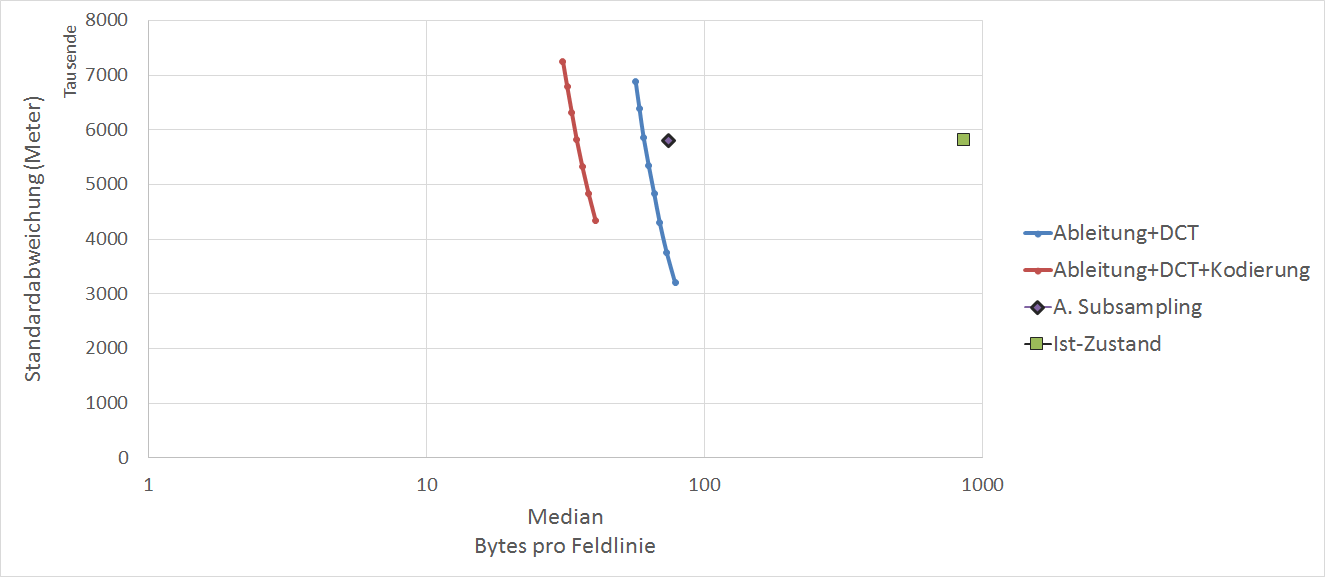
\includegraphics[width=0.8\textwidth,height=6cm,keepaspectratio]{./pictures/resultate/loesung1/loesung1-6/loesung1_6.png}
	\caption{Vergleich der Kompression mit und ohne Byte-Kodierung}
	\label{resultate:loesung1:dct:kodierung}
\end{figure}
\ref{resultate:loesung1:dct:kodierung} zeigt eine deutliche Verbesserung der Kompressionsrate, wenn die Koeffizienten mit der unter \ref{konzept:loesung1:kodierung} beschriebenen Verfahren kodiert werden. Bei ähnlicher Genauigkeit wie der Ist-Zustand braucht diese Variante durchschnittlich $35$ Bytes pro Feldlinie. Bei $1200$ Feldlinien eine ergibt das eine Dateigrösse von $42$ KiByte pro Aufnahme. Im Vergleich zum Ist-Zustand sind die Dateien um das 24 Fache kleiner.\\
[\baselineskip]
Bei der Variante \ref{resultate:dct} war das Problem, dass die Ränder schlecht darzustellen waren. Es stellt sich die Frage, was für Artefakte diese Kompression aufweist.
\begin{figure}[!htbp]
	\center
	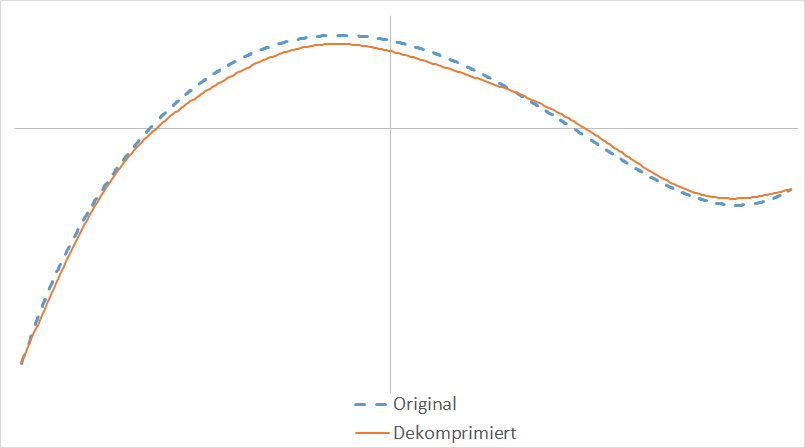
\includegraphics[width=0.8\textwidth,height=6cm,keepaspectratio]{./pictures/resultate/loesung1/loesung1-6/artefakte.png}
	\caption{Artefakte der DCT Kompression der Ableitung}
	\label{resultate:loesung1:dct:byte:artefakte}
\end{figure} 
Im Diagramm der Abbildung\ref{resultate:loesung1:dct:byte:artefakte} ist deutlich zu sehen, dass die Kurve durch die Quantisierung gedämpft wird. Die Maximum der Kurve ist tiefer, sowie das lokale Minima der letzten Halbwelle höher. Der Vorteil dieser Variante ist, dass die resultierende Feldline sehr glatt verläuft. Ohne die Originalkurve währen die Artefakte nicht zu identifizieren.\\
Wenn  die Artefakte \ref{resultate:loesung1:dct:byte:artefakte} und \ref{resultate:loesung0:artefakte} vergleicht, fällt auf, dass die Variante \ref{resultate:dct} die Feldlinie genauer approximiert. Wenn die Ränder besser dargestellt werden, ist es Denkbar, dass die Variante \ref{resultate:dct} wenigere Kosinus-Funktionen braucht für eine ähnlich genaue Approximation.

\subsubsection{Variante: Randbehandlung+DCT+Byte Kodierung} \label{resultate:loesung1:dct:randbeh+byte}
Wieder nur die Diskrete Kosinus Transformation, aber noch mit künstlich erzeugten Punkten\ref{konzept:loesung1:randbehandlung} und der Byte Kodierung\ref{konzept:loesung1:kodierung}.
\begin{figure}[!htbp]
	\center
	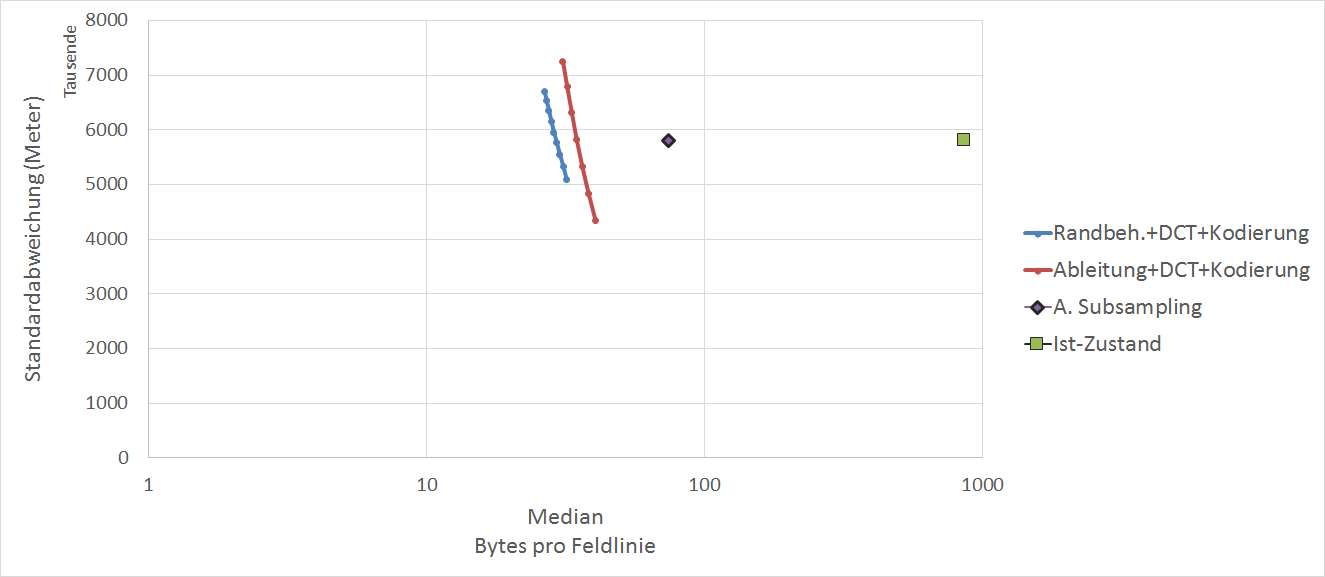
\includegraphics[width=0.8\textwidth,height=6cm,keepaspectratio]{./pictures/resultate/loesung1/loesung1-7/loesung1_7.png}
	\caption{Vergleich der Kompression mit und ohne Byte-Kodierung}
	\label{resultate:loesung1:dct:randbehandlung}
\end{figure}
Das Diagramm der Abbildung \ref{resultate:loesung1:dct:randbehandlung} zeigt den Vergleich der Variante mit Randbehandlung und der Variante der abgeleiteten Feldlinie (beschrieben im Abschnitt \ref{resultate:loesung1:ableitung_dct_kodierung}. Es ist zu erkennen, dass dank der Randbehandlung die Feldlinien mit weniger Bytes ähnlich genau approximiert werden können.\\
[\baselineskip]
Trotz einer vergleichbaren Genauigkeit wie die des Lösungsansatzes unter \ref{resultate:loesung0}, sind auf der JHelioviewer visualisierung deutliche Artefakte zu sehen. Die Abbildung \ref{resultate:loesung1:dct:randbehandlung:jvhartefakte} vergleicht die originalen mit dekomprimierten Feldlinien. Die Dekompression Lässt die Feldlinien um das originale Signal schwingen.
\begin{figure}[!htbp]
	\center
	\frame{
	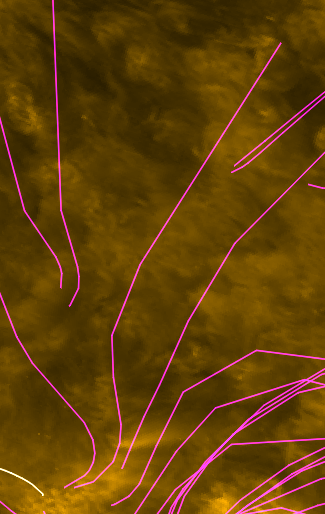
\includegraphics[width=0.8\textwidth,height=6cm,keepaspectratio]{./pictures/resultate/loesung1/loesung1-7/line_good.png}}
		\frame{
	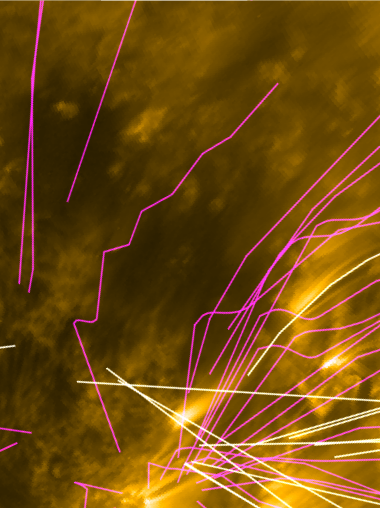
\includegraphics[width=0.8\textwidth,height=6cm,keepaspectratio]{./pictures/resultate/loesung1/loesung1-7/line_bad.png}}
	\caption{Artefakte der Kompression, links sind die originalen Feldlinien, rechts die Dekomprimierten.}
	\label{resultate:loesung1:dct:randbehandlung:jvhartefakte}
\end{figure} 
In diesem Fall scheint die Genauigkeitsmetrik zu versagen: Da die Schwingungen nahe am originalen Signal liegen, bleiben die Abstände klein. Die Approximation ist mathematisch betrachtet genau, aber für das menschliche Auge inakzeptabel.\\
Interessant ist, dass die die Variante der Ableitung beschrieben(\ref{resultate:loesung1:ableitung_dct_kodierung}) ähnliche Artefakte aufweist. In der Abbildung \ref{resultate:loesung1:dct:randbehandlung:jvhartefakte_loesung6} ist ein Vergleich der Original- mit den dekomprimierten Feldlinien dieser Variante zu sehen. Die Artefakte sind deutlich schwächer ausgeprägt. Metrik ist unbrauchbar, Deshalb wurde eine neue Metrik entwickelt, welche unter\ref{testsetup:psnr} beschrieben ist.
\begin{figure}[!htbp]
	\center
	\frame{
	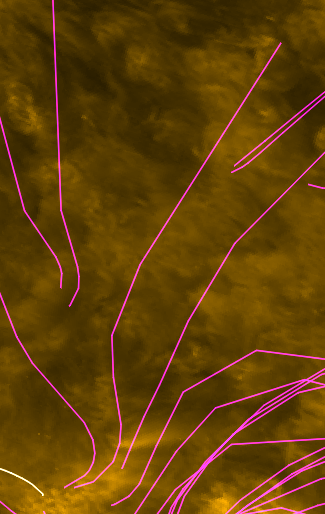
\includegraphics[width=0.8\textwidth,height=6cm,keepaspectratio]{./pictures/resultate/loesung1/loesung1-7/line_good.png}}
		\frame{
	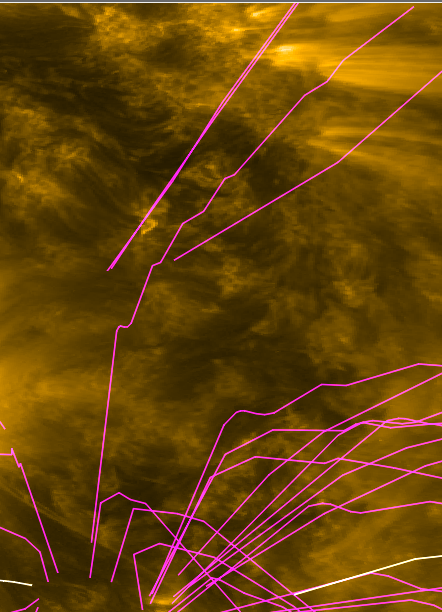
\includegraphics[width=0.8\textwidth,height=6cm,keepaspectratio]{./pictures/testsetup/newalgo//solution6_bad.png}}
	\caption{Artefakte der Kompression, links sind die originalen Feldlinien, rechts die Dekomprimierten der Variante \ref{resultate:loesung1:ableitung_dct_kodierung}.}
	\label{resultate:loesung1:dct:randbehandlung:jvhartefakte_loesung6}
\end{figure} 
